\chapter{Bestanden overzetten}

\section{Bestanden naar de MEGA65 overbrengen}
\label{cha:transferring-files}
\index{SD-kaarten!Bestanden overzetten}

Het schrijven van uw eigen programma's voor de MEGA65 is erg leuk, maar uiteindelijk wilt u ook programma's uitvoeren die door anderen zijn geschreven. Wellicht wilt u ook een reservekopie van uw MEGA65-programma's op uw pc maken om ze veilig te bewaren.

De snelste en betrouwbaarste manier om bestanden tussen uw pc en uw MEGA65 over te zetten is met een Ethernet-kabel.\index{Netwerk!Ethernet} U sluit het ene uiteinde van de kabel aan op de RJ45-aansluiting aan de achterzijde van de MEGA65. U kunt het andere uiteinde aansluiten op de router of switch van uw local area network (LAN), of rechtstreeks op uw pc. U gebruikt software op uw pc om bestandsoverdrachten in beide richtingen te starten: van de pc naar de MEGA65 of van de MEGA65 naar de pc.

Als alternatief kunt u D81-virtuele schijfimages met behulp van een willekeurige pc met een SD-kaartlezer naar uw door de MEGA65 geformatteerde SD-kaart kopiëren, zonder andere speciale hulpmiddelen of software. Uw pc herkent het gegevensgebied van de SD-kaart als een FAT32-partitie. Indien u deze methode gebruikt, dient u zich ervan bewust te zijn dat sommige besturingssystemen van pc's ongewenste neveneffecten kunnen hebben, zoals fragmentatie van bestanden op de SD-kaart of overbodige bestanden die door macOS Finder worden aangemaakt. Deze effecten zijn onschadelijk voor de gegevens, maar kunnen onderhoud vergen om de kaart bruikbaar te houden in de MEGA65. Indien de MEGA65 meldt dat een bestand gefragmenteerd is, kunt u op de gegevenspartitie een defragmentatiehulpmiddel voor pc-schijven gebruiken. Als alternatief kunt u alle bestanden van de SD-kaart naar de pc kopiëren, de SD-kaart in de MEGA65 opnieuw formatteren en de bestanden vervolgens vanaf de pc terugkopiëren.

Het is ook mogelijk om bestanden over te zetten via een JTAG- of UART seriële interface die op het moederbord is aangesloten. Dit is een geavanceerde techniek en wordt niet in deze gebruikershandleiding beschreven. JTAG- of UART Serial-hardware biedt toegang tot een debuginterface die voor sommige programmeurs nuttig kan zijn. JTAG is ook nuttig voor het ontwikkelen van FPGA-cores. Zie voor meer informatie {\it De Mega65 programmeergids.}

De meeste mensen geven de voorkeur aan de Ethernet-methode. Dit hoofdstuk beschrijft hoe u dat doet.

\section{Netwerken begrijpen}

De MEGA65 kan Ethernet gebruiken om verbinding te maken met andere computers in een netwerk, of om verbindingen van andere computers te aanvaarden. Met de juiste programmatuur kan hij via het internet verbinding maken met andere computers.

De Ethernet-hardware van de MEGA65 biedt het lokale netwerk een Media Access Control (MAC)-adres aan.\index{Netwerk!MAC-adres} In tegenstelling tot andere Ethernet-hardware wordt het MAC-adres van de MEGA65 niet in de fabriek toegewezen: het wordt ingesteld in het configuratiehulpprogramma. (Zie hoofdstuk \vref{cha:configuringyourmega}.)

Om bestanden over te zetten, geeft u de MEGA65 opdracht zich beschikbaar te stellen voor binnenkomende verbindingen. Vervolgens gebruikt u op uw pc de M65Connect-app (of een ander hulpprogramma, zoals \texttt{mega65\_ftp}) om een verbinding tot stand te brengen. Het besturingssysteem van uw pc kan om toestemming vragen om het hulpprogramma toegang tot het netwerk te verlenen wanneer u het voor de eerste keer uitvoert. Het hulpmiddel gebruikt UDP-poort 4510 om de eerste verbinding met de MEGA65 tot stand te brengen en gebruikt voor de bestandsoverdrachtssessie een zelf toegewezen IPv6-adres dat op basis van het MAC-adres van de MEGA65 is aangemaakt. Hiervoor moet IPv6 op de netwerkinterface van de pc zijn ingeschakeld, wat in de meeste gevallen de standaardinstelling is.

Als alternatief voor de aansluiting op uw lokale netwerk kunt u de MEGA65, indien uw pc over een Ethernet-aansluiting beschikt, rechtstreeks met een Ethernet-kabel op uw pc aansluiten. Zo vormt u een klein lokaal netwerk zonder toegang tot het internet. De werkwijze voor het overzetten van bestanden is bij een rechtstreekse verbinding dezelfde als bij een verbinding via het lokale netwerk.

\section{M65Connect verkrijgen}
\index{M65Connect-toepassing}

{\bf M65Connect} is een toepassing voor Windows, Mac of Linux die bestandsoverdrachten en andere nuttige functies voor MEGA65-gebruikers mogelijk maakt. De toepassing beschikt over een interface met vensters en bevat tevens commandoregelhulpmiddelen die nuttig zijn bij het programmeren.

Om M65Connect te verkrijgen:

\begin{enumerate}
\item Bezoek de MEGA65 Filehost-website\index{Filehost-website} in een browser: \url{https://files.mega65.org}\item Typ in het zoekveld rechtsboven: ``M65Connect''\item Selecteer de versie van M65Connect voor het besturingssysteem van uw pc.\item Klik op de knop ``Download''.\item Gebruik uw pc om het gedownloade archiefbestand uit te pakken.
\end{enumerate}

\subsection{M65Connect voor Windows}

De Windows-versie van M65Connect staat in de map ``M65Connect'': {\bf M65Connect.exe}. Zoals bij de meeste openbronprogrammatuur het geval is, kan Microsoft Defender weigeren de programmatuur uit te voeren en een dialoogvenster weergeven. Indien dit gebeurt, klikt u op ``More info'' en vervolgens op de knop ``Run anyway'' die verschijnt.

De commandoregelhulpmiddelen staan in een submap met de naam ``M65Connect Resources'', zoals: {\tt M65Connect Resources\textbackslash{}mega65\_ftp.exe}

\subsection{M65Connect voor macOS}

De macOS-versie van M65Connect is een Mac-toepassingsbundel: {\bf M65Connect.app}. Zoals bij de meeste openbronprogrammatuur het geval is, beschouwt macOS het niet als door de ontwikkelaar ondertekend en zal macOS weigeren het uit te voeren. U moet het kenmerk ``quarantine'' verwijderen om de toepassing te kunnen uitvoeren.

In de meeste versies van macOS kunt u het quarantainekenmerk het eenvoudigst verwijderen met een Terminal-opdracht:

\begin{enumerate}
\item Verplaats de M65Connect-app naar uw map Applications.\item Open de Terminal-app, die bij macOS is inbegrepen. U vindt deze in de map Applications, in een submap met de naam Utilities.\item Voer deze opdracht in: {\tt xattr -cr /Applications/M65Connect.app}
\end{enumerate}

U kunt de M65Connect-app nu met een dubbelklik uitvoeren.

De commandoregelhulpmiddelen bevinden zich in de map van de toepassingsbundel, zoals: {\tt /Applications/M65Connect.app/Contents/Resources/mega65\_ftp.osx}

\subsection{M65Connect voor Linux}

De Linuxversie van M65Connect bevindt zich in de map ``M65Connect'': {\bf M65Connect}. Dubbelklik erop om het uit te voeren.

De commandoregelhulpmiddelen staan in een submap met de naam ``M65Connect Resources'', zoals: {\tt M65Connect Resources/mega65\_ftp}

\section{Netwerkluisteren inschakelen}
\index{Netwerk!Luistermodus}

Standaard negeert de MEGA65 alle pogingen van andere computers om er via het netwerk verbinding mee te maken. Programmatuur welke op de MEGA65 draait, kan luisteren naar netwerkverbindingen, doch de MEGA65 doet dit niet uit zichzelf.

Om bestanden met M65Connect over te zetten, dient u de MEGA65 te laten luisteren naar binnenkomende verbindingspogingen van M65Connect. Druk op \specialkey{SHIFT} + \megakey{\pounds} om een netwerkluistersessie in te schakelen. Het stroomlampje knippert afwisselend geel en groen wanneer netwerkluisteren actief is.

\begin{center}
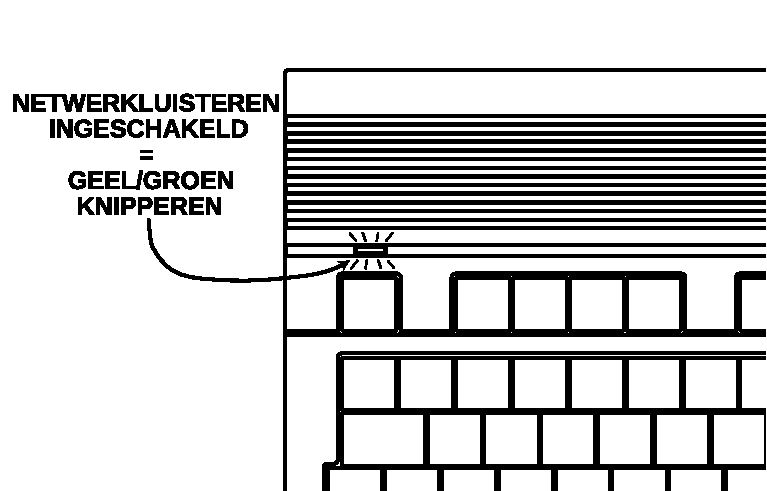
\includegraphics[width=\linewidth]{dutch/images/illustrations/mega65-eth-blink.pdf}
\end{center}

Druk opnieuw op \specialkey{SHIFT} + \megakey{\pounds} om netwerkluisteren uit te schakelen, of reset de computer.

Indien het stroomlampje na het indrukken van \specialkey{SHIFT} + \megakey{\pounds} niet begint te knipperen, moet u mogelijk DIP-schakelaar \#2 op het moederbord instellen. Bij MEGA65-modellen die in 2024 of later zijn gefabriceerd, hoort deze schakelaar in de fabriek ingesteld te zijn. Bij oudere MEGA65-modellen staat deze schakelaar standaard uit.

Om de DIP-schakelaar in te stellen,\index{DIP-schakelaars} opent u de behuizing zoals beschreven in hoofdstuk \vref{cha:setup}. Zoek de DIP-schakelaars op het moederbord en zet DIP-schakelaar \#2 in de positie ``on''. Zoek naar markeringen op de schakelaars om schakelaar \#2 en de richting ``on'' te herkennen. (De oriëntatie van uw DIP-schakelaars kan van dit diagram afwijken.)

\begin{center}
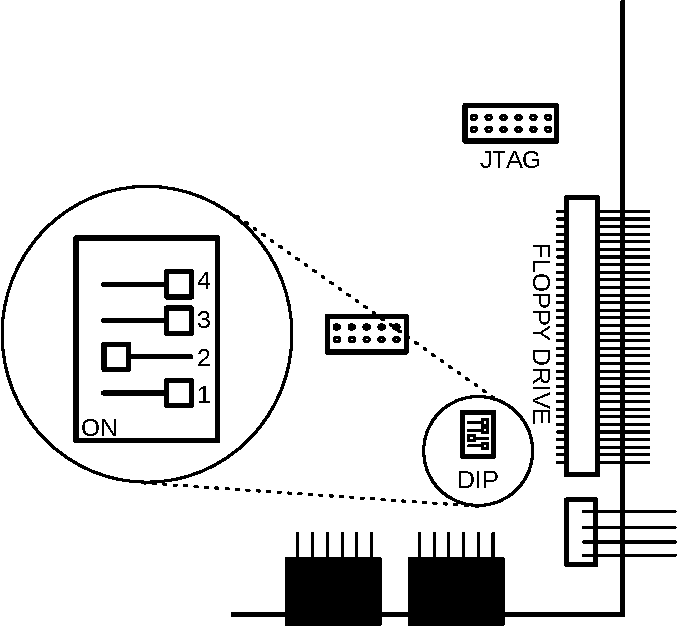
\includegraphics[width=\linewidth]{images/illustrations/mega65-dip2.pdf}
\end{center}

U kunt DIP \#2 gerust in deze positie laten staan voor normaal gebruik.


\section{Bestanden overzetten}

Om bestanden over te zetten, start u een bestandsoverdrachtssessie met de toepassing M65Connect of het commandoregelhulpmiddel {\tt mega65\_ftp}. Dit hulpmiddel maakt verbinding met de MEGA65 en uploadt een bestandsoverdrachtclient voor gebruik tijdens de sessie. Wanneer u de sessie beëindigt, reset de MEGA65.

Het starten van een bestandsoverdrachtssessie reset de MEGA65. Sla eventuele programma's of gegevens op voordat u verdergaat.

\underline{OPMERKING}: Indien u het geheugen wist door de computer te resetten, vergeet dan niet om netwerkluisteren opnieuw in te schakelen: druk op \specialkey{SHIFT} + \megakey{\pounds} en zorg dat het stroomlampje knippert.

\subsection{Bestanden overzetten met M65Connect}
\index{M65Connect-toepassing}

M65Connect detecteert automatisch of de MEGA65 naar verbindingen luistert. Open M65Connect en schakel vervolgens de netwerkluistersessie op de MEGA65 in. M65Connect meldt een status van "Connected to MEGA65 via LAN". M65Connect schakelt daarna in het venster diverse knoppen in, waaronder de {\bf PRG}- en {\bf SD Card}-knoppen.

\begin{center}
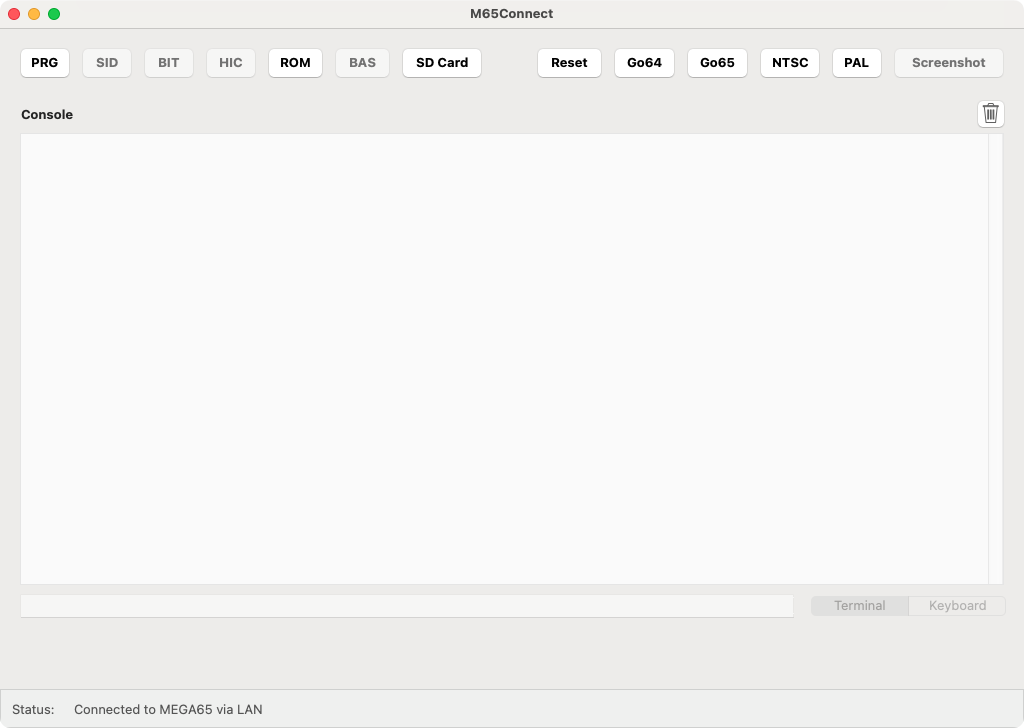
\includegraphics[width=\linewidth]{images/m65connect_macos.png}
\end{center}

Indien M65Connect een status van "Not connected to MEGA65" meldt, controleer dan het volgende:

\begin{itemize}
\item De MEGA65 en de pc zijn op hetzelfde netwerk aangesloten of rechtstreeks op elkaar via een netwerkkabel.\item De MEGA65 bevindt zich in de netwerkluistermodus met een knipperend stroomlampje.\item Open in M65Connect het menu Settings en selecteer Connections. Het veld "LAN Port" hoort een IPv6-adres te bevatten. Indien dat niet het geval is, wacht dan enkele seconden of klik op de knop "Autodetect LAN Port".
\end{itemize}

Klik op de knop {\bf SD Card} om een bestandsoverdrachtssessie te starten. Het SD Card Manager-venster gaat open.

\underline{OPMERKING}: Het starten van een bestandsoverdrachtssessie reset de MEGA65 om het bestandsoverdrachtshulpprogramma te laden. Zorg ervoor dat u eventuele gegevens op de MEGA65 hebt opgeslagen voordat u de sessie start.

\begin{center}
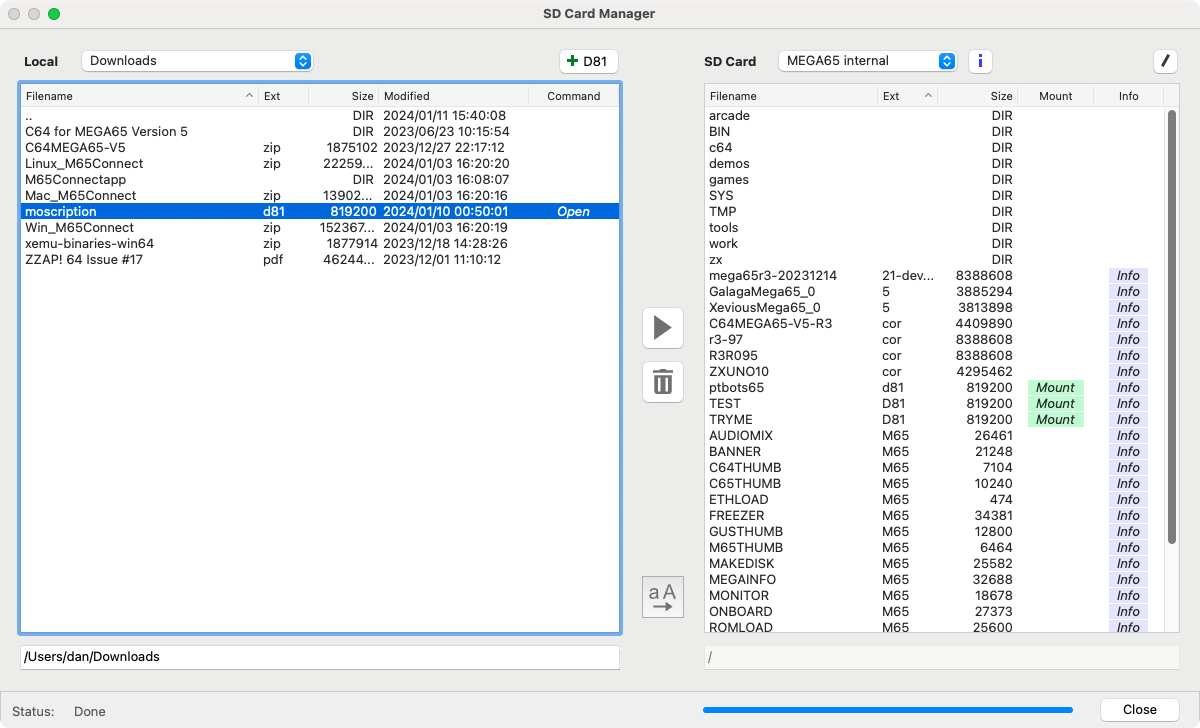
\includegraphics[width=\linewidth]{images/m65connect_files.png}
\end{center}

Gebruik het linkerdeelvenster om door de bestanden op uw pc te navigeren en het rechterdeelvenster om door de bestanden op de SD-kaart van de MEGA65 te navigeren. Selecteer het bestand en klik daarna op de pijlknop om het over te zetten. De knop geeft de richting aan waarin het bestand wordt overgezet.

U kunt M65Connect ook gebruiken om D81-schijfimages aan te maken en bestanden van en naar D81-schijfimages te kopiëren. Zoek een D81-schijfimage op uw pc of klik op de knop {\bf + D81} om er een aan te maken. Klik daarna in de bestandsverkenner op de opdracht "Open" om het schijfimage in het linkerdeelvenster te openen. Zet bestanden met de pijlknop over van en naar het schijfimage. Klik op de knop {\bf X} in de rechterbovenhoek om terug te keren naar de bestandsverkenner.

Klik op de knop {\bf Close} om de bestandsoverdrachtssessie te beëindigen en het SD Card Manager-venster te sluiten. Dit reset de MEGA65.

\subsection{Het commandoregelhulpmiddel mega65\_ftp}
\index{mega65\_ftp-commando@\texttt{mega65\_ftp-commando}}

Het commandoregelhulpmiddel {\tt mega65\_ftp} start een bestandsoverdrachtssessie met de MEGA65. Het kan interactief in de terminal draaien en meerdere bestandsoverdrachtopdrachten aanvaarden, of niet-interactief draaien met deze opdrachten als argumenten.

Om een interactieve bestandsoverdrachtssessie te starten, voert u de opdracht {\tt mega65\_ftp} uit en geeft u daarbij het argument {\tt -e} mee om aan te geven dat u een Ethernet-verbinding wilt gebruiken.

\underline{OPMERKING}: Het starten van een bestandsoverdrachtssessie reset de MEGA65 om het bestandsoverdrachtshulpprogramma te laden. Zorg ervoor dat u eventuele gegevens op de MEGA65 hebt opgeslagen voordat u de sessie start.

\begin{verbatim}
% mega65_ftp -e
\end{verbatim}

Het hulpprogramma uploadt de bestandsoverdrachtclient en u ziet de client op de MEGA65 draaien. Indien er niets gebeurt, drukt u op Ctrl-C (op de pc) om de overdracht af te breken en controleert u daarna nogmaals of de MEGA65 verbonden is en of netwerkluisteren is ingeschakeld.

Zodra de verbinding tot stand is gekomen, ziet de prompt voor bestandsoverdrachtopdrachten er ongeveer zo uit:

\begin{verbatim}
MEGA65 SD-Card:/>
\end{verbatim}

Om de sessie te beëindigen, gebruikt u de opdracht {\tt exit}. Het hulpprogramma sluit af, u keert terug naar de shellprompt en de MEGA65 reset.

\begin{verbatim}
MEGA65 SD-Card:/> exit
%
\end{verbatim}

Hieronder volgen enkele nuttige opdrachten die u tijdens de bestandsoverdrachtssessie kunt gebruiken. Gebruik de opdracht {\tt help} om een volledige lijst van de beschikbare opdrachten te zien.

\begin{center}
\begin{tabular}{|l|l|}
\hline
{\bf Opdracht} & {\bf Omschrijving} \\
\hline
{\tt put {\it bestandsnaam}} & Verstuurt een bestand van de pc naar de MEGA65. \\
\hline
{\tt get {\it bestandsnaam}} & Haalt een bestand op van de MEGA65 en plaatst het op de pc. \\
\hline
{\tt dir} & Toont een lijst van de mappen van de SD-kaart van de MEGA65. \\
\hline
{\tt ldir} & Toont een lijst van de huidige lokale werkmap. \\
\hline
{\tt mkdir {\it bestandsnaam}} & Maakt een submap aan op de SD-kaart van de MEGA65. \\
\hline
{\tt cd {\it bestandsnaam}} & Wijzigt de huidige werkmap op de SD-kaart van de MEGA65. \\
\hline
{\tt lcd {\it bestandsnaam}} & Wijzigt de huidige lokale werkmap. \\
\hline
{\tt help} & Toont een lijst met beschikbare opdrachten. \\
\hline
{\tt exit} & Beëindigt de bestandsoverdrachtssessie. \\
\hline
\end{tabular}
\end{center}

Om opdrachten van {\tt mega65\_ftp} aan te roepen zonder een interactieve prompt te starten, geeft u het argument {\tt -c} één keer per opdracht mee:

\begin{verbatim}
% mega65_ftp -e -c 'put mydisk.d81' -c 'exit'
\end{verbatim}

Het hulpprogramma start een sessie, voert de opdrachten uit en stopt vervolgens. Zorg ervoor dat u de opdracht {\tt exit} als laatste opdracht invoert om de MEGA65 te resetten, of reset de MEGA65 handmatig nadat de bestandsoverdracht is voltooid.